\section{Auswertung}
\label{sec:Auswertung}

\subsection{Bestimmung der Untergrundrate}

Die Messung eribt die in Tabelle \ref{tab:Untergrundrate} aufgeführten Werte. Das Messintervall beträgt $\SI{300}{\second}$. 
\begin{table}
    \centering
    \caption{Messwerte zur Bestimmung der Untergrundrate.}
    \label{tab:Untergrundrate}
    \begin{tabular}{c}
        \toprule
        $N^*_\text{U}$ \\
        \midrule
        129 \\
        143 \\
        144 \\
        136 \\
        139 \\ 
        126 \\
        158 \\
        \bottomrule
    \end{tabular}
\end{table}
Dadurch ergibt sich ein experimenteller Wert von 
\begin{equation*}
    N^*_\text{U}=\num{139+-12}
\end{equation*}
für die Anzahl der Impulse, die durch den Untergrund bestimmt sind, und 
\begin{equation}
    N_\text{U}=\SI{0.464+-0.038}{\per\second}
    \label{eqn:Untergrund}
\end{equation}
für die entsprechende Impulsrate.
Der Mittelwert und die experimentelle Messunsicherheit berechnen sich hier über 
\begin{equation*}
    \bar{x}=\sum_{i=1}^N x_i \quad \text{und}
\end{equation*}
\begin{equation*}
    \Delta x = \sqrt{\frac{1}{N-1} \sum_{i=1}^N (x_i-\bar{x})^2}
\end{equation*}

\subsection{Vanadium}

\subsection{Rhodium}

In Tabelle werden die benötigten Daten zur Auswertung des Zerfalls von Rhodium aufgeführt. 
Im ersten Schritt wird der aus der ersten Messung ermittelte Wert für den Untergrund bezogen auf $\SI{15}{\second}$ (nicht auf $\SI{300}{\second}$) $\bar{N}_\text{U}=139\cdot \sfrac{15}{300}\approx 7$ von den Messwerten des Zerfalls von Rhodium abgezogen. 
Das ergibt die hier mit $N_\text{Rh}$ bezeichnete Messreihe. 
Der Fehler der Impulse ist poisson-verteilt, weshalb sich ein Fehler von $\Delta N_\text{Rh}=\sqrt{N_\text{Rh}}$ ergibt. 
Die verwendete Messzeit beträgt hier, wie an den Messwerten zu erkennen ist, $\SI{15}{\second}$. 
\begin{table}
    \centering
    \caption{Die Zerfallswerte zum Rhodium.}
    \label{tab:MessRh}
    \begin{tabular}{S[table-format=3.0] S[table-format=3.0] S[table-format=2.0] S[table-format=3.0] S[table-format=2.0] S[table-format=1.0]}
        \toprule
        $t\,/\,\si{\second}$ & $N_\text{Rh}$ & $\Delta N_\text{Rh}$ & $t\,/\,\si{\second}$ & $N_\text{Rh}$ & $\Delta N_\text{Rh}$  \\
        \midrule
        15  & 660 & 26 & 345 & 29 & 5 \\
        30  & 578 & 24 & 360 & 31 & 5 \\
        45  & 467 & 22 & 375 & 27 & 5 \\
        60  & 392 & 20 & 390 & 33 & 5 \\
        75  & 297 & 17 & 405 & 14 & 4 \\
        90  & 246 & 16 & 420 & 28 & 5 \\
        105 & 206 & 14 & 435 & 26 & 5 \\
        120 & 166 & 12 & 450 & 29 & 5 \\
        135 & 145 & 12 & 465 & 13 & 4 \\
        150 & 119 & 11 & 480 & 17 & 4 \\
        165 & 104 & 10 & 495 & 23 & 5 \\
        180 & 85  &  9 & 510 & 23 & 5 \\
        195 & 72  &  8 & 525 & 19 & 4 \\
        210 & 67  &  8 & 540 & 21 & 5 \\
        225 & 53  &  7 & 555 & 16 & 4 \\
        240 & 45  &  7 & 570 & 13 & 4 \\
        255 & 49  &  7 & 585 & 21 & 5 \\
        270 & 46  &  7 & 600 & 10 & 3 \\
        285 & 34  &  6 & 615 & 19 & 4 \\
        300 & 29  &  5 & 630 & 12 & 3 \\
        315 & 30  &  5 & 645 &  6 & 2 \\
        330 & 25  &  5 & 660 & 10 & 3 \\
        \bottomrule
    \end{tabular}
\end{table}
\begin{figure}
    \centering
    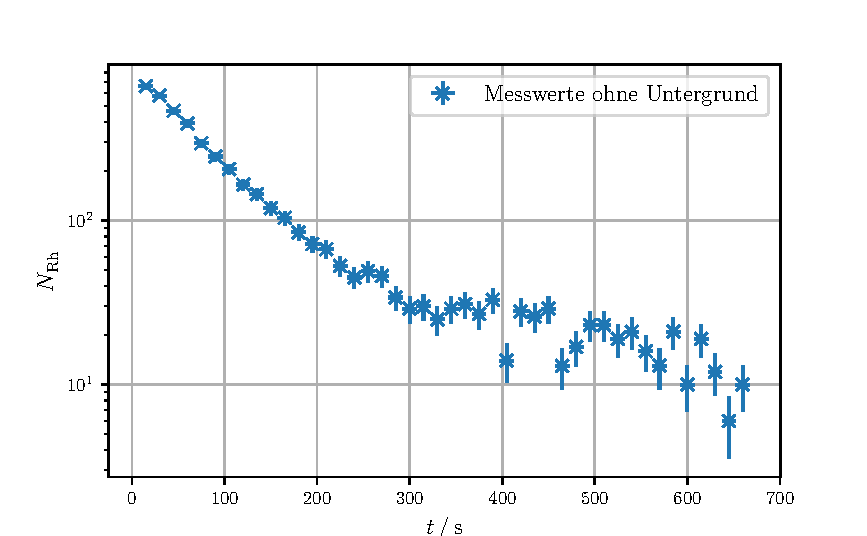
\includegraphics[width=0.8\textwidth]{plots/Rhodium.pdf}
    \caption{Gemessene Zerfallskurve von Rhodium.}
    \label{fig:RhodiumMess}
\end{figure}
Zuerst wird der langsame Zerfall untersucht, wie in Abschnitt \ref{sub:keineAhnung} beschrieben. 
Die Zeit, ab der nur noch der zweite Zerfall ausschlaggebend ist, wird anhand von Abbildung \ref{fig:RhodiumMess} zu $t^*=\SI{330}{\second}$ festgelegt.
Für die Messwerte $t>t^*$ wird nun analog zur Gleichung \eqref{eqn:linRegr} eine lineare Ausgleichsgerade mithilfe von 
\cite{scipy} und \cite{uncertainties} berechnet, die mit der Methode der kleinsten Quadrate rechnet und die Messfehler der Messwerte berücksichtigt. 

Die Geradenparameter der beiden Zerfälle und die sich daraus ergebende Totzeit $\tau$ sind übersichtlich in Tabelle \ref{tab:Denkdirwasaus} zusammengestellt. 
\begin{table}
    \centering
    \caption{Die sich aus der Ausgleichsrechnung für Rhodium ergebenden Parameter.}
    \label{tab:Denkdirwasaus}
    \begin{tabular}{l c c c c}
        \toprule
         & $m\,/\SI{e-3}{\second\tothe{-1}}$ & $b$ & $\lambda\,/\,\si{\second\tothe{-1}}$ & $\tau\,/\,\si{\second}$ \\
        \midrule
        langsam & \num{-2.53+-0.53} & \num{4.28+-0.25} & \num{2.53+-0.53} & \num{270+-60}   \\
        schnell & \num{-17.7+-0.6}  & \num{6.78+-0.07} & \num{17.7+-0.6}  & \num{39.3+-1.4} \\
        \bottomrule
    \end{tabular}
\end{table}
Zur Veranschaulichung der Vorgänge bei der Fehlerrechnung und der Größe der Messfehler dienen die Abbildungen \ref{fig:RHlin} und \ref{fig:Rhodium_kombi}. 
\begin{figure}
    \begin{subfigure}{0.5\textwidth}
        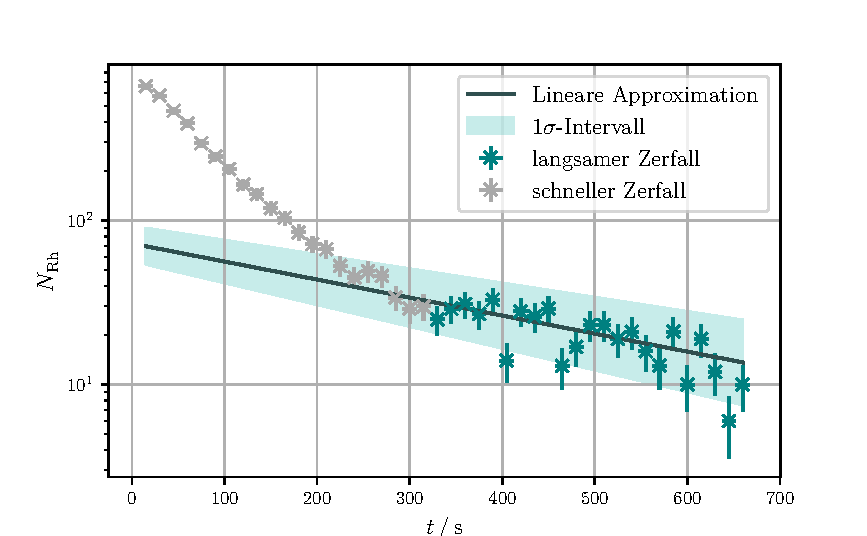
\includegraphics[width=0.95\textwidth]{plots/Rhodium_langsam.pdf}
        \subcaption{Die lineare Regression zum langsamen Zerfall.}
    \end{subfigure}
    \begin{subfigure}{0.5\textwidth}
        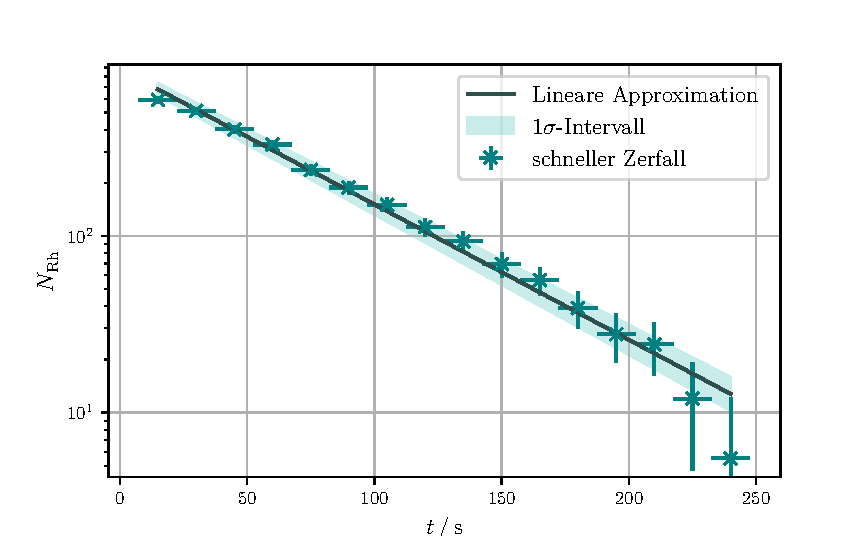
\includegraphics[width=0.95\textwidth]{plots/Rhodium_schnell.pdf}
        \subcaption{Die lineare Regression zum schnellen Zerfall.}
    \end{subfigure}
    \caption{Beide linearen Regression zum Rhodium-Präparat.}
    \label{fig:RHlin}
\end{figure}
\begin{figure}
    \centering
    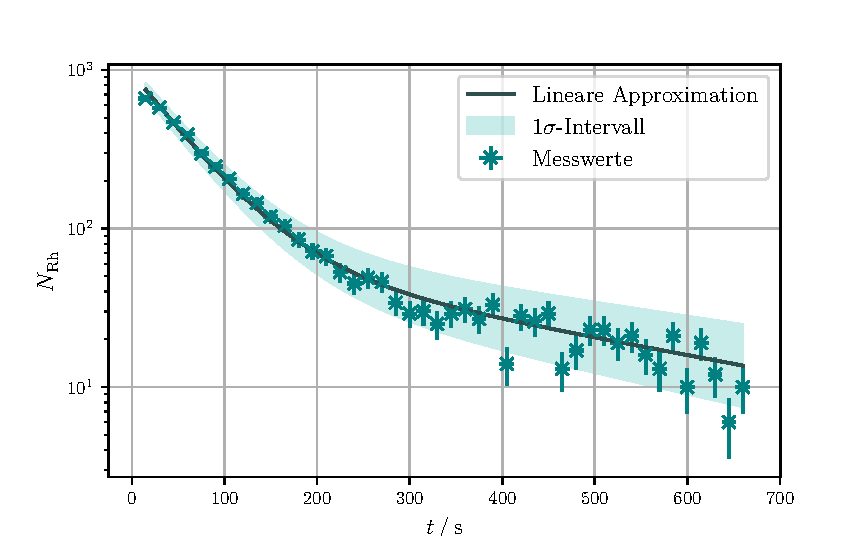
\includegraphics[width=\textwidth]{python/Rhodium_kombi.pdf}
    \caption{Gesamtdarstellung der beiden Zerfallvorgänge.}
    \label{fig:Rhodium_kombi}
\end{figure}